% ============================================================
% main_cn.tex — 论文中文版
% 标题：基于心肺运动试验汇总指标的老年高血压患者运动安全分层框架：
%       条件分位参考建模与不确定性量化
%
% 文档类：ctexart；编译链：xelatex + bibtex
% 参考文献：GB/T 7714-2015（gbt7714 本地安装）
%
% 编译方法：
%   xelatex main_cn.tex
%   bibtex main_cn
%   xelatex main_cn.tex
%   xelatex main_cn.tex
%
% 注意：gbt7714 包需要本地安装。若系统未安装，请从 CTAN 下载：
%   curl -sL "https://mirrors.ctan.org/biblio/bibtex/contrib/gbt7714.zip" \
%        -o /tmp/gbt7714.zip
%   cd /tmp && unzip gbt7714.zip -d gbt7714_extracted
%   cd /tmp/gbt7714_extracted/gbt7714 && latex gbt7714.ins
%   cp *.sty *.bst /path/to/paper/
% ============================================================

\documentclass[12pt, a4paper]{ctexart}

% ------ 基础包 ------
\usepackage{geometry}
\geometry{left=2.5cm, right=2.5cm, top=3cm, bottom=3cm}
\usepackage{setspace}
\onehalfspacing

% ------ 参考文献（GB/T 7714-2015）------
\usepackage[super,square,sort&compress]{natbib}
% 尝试 gbt7714；若未安装则注释掉以下两行改用标准样式
\usepackage{gbt7714}
\bibliographystyle{gbt7714-numerical}

% ------ 图表 ------
\usepackage{graphicx}
\usepackage{booktabs}
\usepackage{array}
\usepackage{multirow}
\usepackage{caption}
\captionsetup{font=small, labelfont=bf}

% ------ 数学 ------
\usepackage{amsmath}
\usepackage{amssymb}

% ------ 颜色与链接 ------
\usepackage[dvipsnames]{xcolor}
\usepackage[hidelinks]{hyperref}

% ------ 其他 ------
\usepackage{enumitem}
\usepackage{float}

% ------ 元数据 ------
\title{基于心肺运动试验汇总指标的老年高血压患者运动安全分层框架：\\
\large 条件分位参考建模与不确定性量化}

\author{\textcolor{red}{TODO: 作者姓名}$^{1}$\\
\small$^{1}$\textcolor{red}{TODO: 单位名称}}

\date{2026年4月}

% ============================================================
\begin{document}
\maketitle

% ------ 摘要 ------
\begin{abstract}
\textbf{背景与目的：}
心肺运动试验（CPET）是运动安全评估的金标准，CPET 汇总指标同时反映慢性心肺储备不足、
通气效率降低及运动中即时血流动力学异常三类不同性质的风险信息。
若将这三类信息混合为单一标签，则会引起概念混淆与循环依赖，
现有欧美参考方程在中国老年高血压患者中存在系统性适用性缺陷，
且现有框架均强制给出确定性分类，未对评估的不确定性加以明确标识。
本研究旨在基于 3,232 例老年高血压患者的 CPET 汇总指标，
构建以表型负担评分为核心、以血流动力学不稳定覆盖规则为安全保障、
并明确量化评估不确定性的运动安全分层框架。

\textbf{方法：}
回顾性单中心研究（N=3,232例，2015—2023年），采用高血压既往史（HTN）$\times$ 运动性高血压（EHT）2$\times$2 设计。
分析流程分四层：
（1）条件分位参考建模（年龄自然三次样条 + 性别 + 运动方案；
$\tau \in \{0.10, 0.25, 0.50, 0.75, 0.90\}$）；
（2）双域表型负担评分（Reserve 域：VO$_2$peak、无氧阈 VO$_2$、O$_2$脉搏、峰值METs；
Ventilatory 域：$V_E/V_{\text{CO}_2}$ slope、OUES；
各变量三级负担；等权域聚合）；
（3）不稳定覆盖规则（严重不稳定强制高危；轻度不稳定将低危升为中危）；
（4）四分量置信度引擎（字段完整度、努力程度、参考一致性、结局一致性加权；
低置信度样本标记为不确定层）。
以 ElasticNet Logistic 回归（嵌套交叉验证）进行外部结构效度锚定验证。

\textbf{结果：}
本地化条件分位参考将 VO$_2$peak $R^2$ 从0.298提升至0.392，
O$_2$脉搏 $R^2$ 从0.200提升至0.511；
欧美参考方程均呈 $R^2<0$（最大偏差$-$11.85 mL/kg/min）。
参考正常子集（N=903）低危比例69.2\%、高危比例10.2\%，
满足预设方法学质量标准。
全量样本（N=3,232）最终安全分层：低危19.7\%、中危25.6\%、高危29.7\%、不确定层24.9\%；
高置信度样本占33.0\%。
结构效度验证：最终安全分层对临床结局替代指标阳性率呈严格单调梯度
（低危14.0\% $<$ 中危15.1\% $<$ 高危18.0\%），方向正确，满足预设方法学质量标准。
外部锚定模型交叉验证 AUC 0.564（$\pm$0.016），测试集 AUC 0.608，
处于 CPET 汇总指标可提取信息量的合理范围。

\textbf{结论：}
本研究建立了一套将慢性心肺储备表型与运动中即时血流动力学不稳定事件严格分开评估、
以不确定性量化取代强制分类的 CPET 运动安全分层框架，
为中国老年高血压患者提供了可复现的 CPET 安全评估方法，
并为后续逐呼吸波形分析研究提供了明确的目标人群筛选依据。

\textbf{关键词：}心肺运动试验；表型负担评分；运动安全分层；不稳定覆盖规则；
置信度量化；不确定性输出；条件分位参考；中国老年高血压
\end{abstract}

% ============================================================
\section{引言}
% ============================================================

全球老龄化背景下，心血管疾病（CVD）是老年人致残致死的首要原因\cite{WHO2023}。
运动康复在 CVD 患者中具有明确的心肺功能改善和预后获益\cite{Piepoli2016,Thomas2019}，
但运动诱发的不良事件风险——尤其是血流动力学不稳定
（运动性高血压、高血压危象）——制约了老年高血压患者运动处方的精准推广\cite{Myers2013}。
心肺运动试验（CPET）是评估运动安全性的金标准\cite{Balady2010,Guazzi2012}，
在中国临床人群中的安全性已由大样本研究证实\cite{Xiangya2021,SunXG2022consensus}，
但如何基于 CPET 汇总指标构建可解释、可复现的安全分层框架，仍有三个关键方法学缺口。

概念混淆是首要方法学挑战。
运动安全涉及"慢性储备不足"（Reserve 表型）与"即时血流动力学不稳定"（Instability 信号）
两类本质不同的风险机制。将二者以等权或数据驱动权重混合为单一评分，
或以临床结局替代指标作为主标签反向推导区间边界，均将导致概念混淆和循环依赖\cite{Ross2024}。
现有 CPET 复合评分（CPX score\cite{Gorodeski2008cpx,CPXvalidation2013}、
MECKI\cite{MECKI2023}）虽已验证预后价值，但主要基于心衰人群和结局驱动回归，
难以直接迁移至中国老年高血压患者的安全分层语境。

参考方程的人群特异性局限是第二个挑战。
欧美参考方程（Wasserman \& Hansen 1999\cite{Wasserman1999}；
Koch et al. 2009\cite{Koch2009}）在中国老年高血压患者中系统失效（$R^2<0$）。
中国本土参考值研究（X-ET 项目\cite{XET2021}；Wang et al.\cite{WangCycle2022}；
Huang et al.\cite{HuangTreadmill2024}；PUTH 方程\cite{PUTHCycle2025}）
提供了宝贵的中国特异性参考，但通常为单方程形式，未纳入年龄-方案交互效应。
FRIEND 系列（2015/2022\cite{FRIEND2016cycle,FRIEND2022}）建立了体系化分位参考框架，
但尚缺乏针对老年高血压合并 EHT 亚群的条件分位参考。

不确定性的明确处理是第三个缺口。
CPET 汇总指标本身存在固有的信息量上限：努力程度不充分、核心字段缺失、
内外参考一致性差均会降低分层可信度。
现有框架通常强制给出确定性分类，未区分"高置信度低危（6个核心字段完整）"
与"仅因字段缺失而默认低负担"的本质差异。
预测模型透明度标准（TRIPOD+AI\cite{TRIPODAI2024}；
PROBAST+AI\cite{PROBASTAI2025}）明确要求对模型边界和不确定性进行明确声明。

本研究旨在弥合上述三个缺口，以 3,232 例老年高血压患者的 CPET 汇总指标为基础，
构建运动安全分层框架。
以条件分位参考模型替代传统单点回归方程，实现个性化参考建模；
以三级负担转换替代连续评分混合，实现表型量化；
以独立覆盖规则处理即时不稳定信号，实现双域分离；
以置信度引擎明确量化评估不确定性，实现如实方法学表达。
本框架定位为方法学工具，为后续逐呼吸波形分析研究提供明确的目标人群筛选标准。

% ============================================================
\section{方法}
% ============================================================

\subsection{研究人群与设计}

本研究为单中心回顾性队列研究，纳入2015年至2023年间完成 CPET 检查的老年患者（$\geq$60岁），
共3,232例，其中26例（0.8\%）存在质量控制标记，采用标记保留法纳入分析。
研究采用 HTN 既往史（有/无）$\times$ EHT 反应（有/无）的 2$\times$2 分层设计
（表~\ref{tab:cohort_design}）。
本研究经伦理委员会批准（批准号：\textcolor{red}{TODO: 填写批准号}），
回顾性设计，豁免知情同意，数据已脱敏处理。

\begin{table}[htbp]
\centering
\caption{HTN$\times$EHT 2$\times$2 队列设计}
\label{tab:cohort_design}
\begin{tabular}{lccc}
\toprule
队列 & 代码 & N（标记保留）& 说明 \\
\midrule
对照/非HTN & CTRL & 1,858 & 无既往HTN史，无EHT \\
既往HTN，无EHT & HTN-NoEHT & 738 & 有HTN史，运动试验中无EHT \\
既往HTN，合并EHT & HTN-EHT & 277 & 有HTN史，运动试验中有EHT \\
仅EHT & EHT-Only & 359 & 无HTN史，运动试验中有EHT \\
\midrule
合计 & & 3,232 & \\
\bottomrule
\end{tabular}
\end{table}

\subsection{变量角色分配}

\textbf{临床结局替代指标}（clinical outcome proxy）操作性定义：
运动试验总体结果（阳性/可疑阳性/阴性），
由监督医师基于心电图变化（ST段压低/室性心律失常等）、
血流动力学反应（峰值血压异常升高/异常降低）、
症状（胸痛、呼吸困难）及运动耐量综合判读后赋予。
本研究将阳性与可疑阳性合并为"阳性"，阴性为"阴性"，形成二元结局。
临床结局替代指标仅在最终安全分层确定后作为外部验证变量使用，
严禁用于定义分层边界（见表~\ref{tab:variable_roles}，验证变量角色）。

本研究明确将 CPET 变量分为四类，防止概念混淆（表~\ref{tab:variable_roles}）。

\begin{table}[htbp]
\centering
\small
\caption{CPET 变量角色分配}
\label{tab:variable_roles}
\begin{tabular}{lll}
\toprule
角色类型 & 变量 & 用途 \\
\midrule
表型变量（Reserve 域）& VO$_2$peak、无氧阈 VO$_2$、O$_2$脉搏峰值、峰值METs & 负担评分 \\
表型变量（Ventilatory 域）& $V_E/V_{\text{CO}_2}$ slope、OUES & 负担评分 \\
不稳定变量 & EHT状态、峰值收缩压、峰值舒张压、O$_2$脉搏轨迹 & 覆盖规则（仅） \\
验证变量 & 临床结局替代指标、队列编码 & 外部锚定验证（仅） \\
\bottomrule
\end{tabular}
\\[1ex]
{\footnotesize 验证变量仅在最终安全分层确定后使用，严禁用于定义分层边界。}
\end{table}

\subsection{参考正常子集}

参考正常子集（Reference Subset）是本框架的核心锚点，定义为：
CTRL 组（无HTN史、无EHT），VO$_2$peak\%pred $\geq$70\%，
$V_E/V_{\text{CO}_2}$ slope $\leq$30，无EHT，峰值心率 $\geq$85\% 最大预测心率。
以此定义筛选严格参考子集（N $\approx$ 900），
以及宽松参考子集（仅要求 CTRL 组，N $\approx$ 969）用于敏感性分析。
严格参考子集用于条件分位模型拟合和表型负担切点估计。

\subsection{条件分位参考模型}

以严格参考子集拟合各变量的条件分位模型，
覆盖 $\tau \in \{0.10, 0.25, 0.50, 0.75, 0.90\}$ 五个分位点。
模型使用线性分位数回归，协变量为年龄自然三次样条基函数与性别、方案指示变量的并置：

\begin{equation}
\label{eq:quantile}
Q_\tau(Y \mid \mathbf{z}) = \boldsymbol{\beta}_\tau^\top
\bigl[\mathbf{s}(\text{age};\, K{=}5) \oplus \mathbf{d}_{\text{sex}}
\oplus \mathbf{d}_{\text{protocol}}\bigr]
\end{equation}

其中 $\mathbf{s}(\cdot;\, K)$ 为自然三次样条基函数（$K$ 个内部节点，捕捉年龄的非线性效应），
$\mathbf{d}$ 为指示变量，$\oplus$ 表示特征向量并置。
参数 $\hat{\boldsymbol{\beta}}_\tau$ 通过最小化 pinball 损失估计：

\begin{equation}
\label{eq:pinball}
\hat{\boldsymbol{\beta}}_\tau = \arg\min_{\boldsymbol{\beta}}
\sum_{i=1}^{n} \rho_\tau\bigl(Y_i - \boldsymbol{\beta}^\top \mathbf{z}_i\bigr),
\quad \rho_\tau(u) = u\bigl(\tau - \mathbf{1}_{u < 0}\bigr)
\end{equation}

单调性约束通过对每个样本的五个分位预测值施加排序约束保证，
确保 $\hat{Q}_{0.10} \leq \hat{Q}_{0.25} \leq \hat{Q}_{0.50}
\leq \hat{Q}_{0.75} \leq \hat{Q}_{0.90}$ 严格成立，踏车与平板方案分别建立独立分位参考。

\subsection{表型负担评分}

\subsubsection{变量级负担转换}

对每个表型变量，基于其条件分位参考值将连续量转换为三级负担（表~\ref{tab:burden_rules}）：

\begin{table}[htbp]
\centering
\small
\caption{表型变量负担转换规则}
\label{tab:burden_rules}
\begin{tabular}{llccc}
\toprule
变量 & 方向 & 负担=0（正常）& 负担=0.5（临界）& 负担=1.0（异常）\\
\midrule
VO$_2$peak & 越高越好 & $\geq$q25 & [q10, q25) & $<$q10 \\
无氧阈 VO$_2$ & 越高越好 & $\geq$q25 & [q10, q25) & $<$q10 \\
O$_2$脉搏峰值 & 越高越好 & $\geq$q25 & [q10, q25) & $<$q10 \\
峰值METs & 越高越好 & $\geq$q25 & [q10, q25) & $<$q10 \\
$V_E/V_{\text{CO}_2}$ slope & 越低越好 & $\leq$q75 & (q75, q90] & $>$q90 \\
OUES & 越高越好 & $\geq$q25 & [q10, q25) & $<$q10 \\
\bottomrule
\end{tabular}
\\[1ex]
{\footnotesize 字段缺失时，该变量负担记为缺失，域内均值以可用字段计算；
Reserve 域须至少2个有效字段，Ventilatory 域须至少1个有效字段。}
\end{table}

\subsubsection{域聚合与综合评分}

Reserve 域负担 $B_R$ 为四个 Reserve 变量负担的域内均值；
Ventilatory 域负担 $B_V$ 为两个 Ventilatory 变量负担的域内均值。
综合表型负担评分：

\begin{equation}
\label{eq:plab}
P_{\text{lab}} = 0.5 \times B_R + 0.5 \times B_V
\end{equation}

$P_{\text{lab}} \in [0, 1]$，0 为无负担，1 为最大负担。
等权设计避免了对结局驱动的参数优化的依赖。
以严格参考子集上 $P_{\text{lab}}$ 分布的 P75 和 P90 为切点，
分别定义低危/中危界和中危/高危界，得到表型负担分层 $Z_{\text{ph}}$：

\begin{equation}
\label{eq:phenotype_zone}
Z_{\text{ph}} =
\begin{cases}
\text{低危}  & P_{\text{lab}} \leq P_{75}^{\text{ref}} \\
\text{中危} & P_{75}^{\text{ref}} < P_{\text{lab}} \leq P_{90}^{\text{ref}} \\
\text{高危}    & P_{\text{lab}} > P_{90}^{\text{ref}}
\end{cases}
\end{equation}

\subsection{不稳定覆盖规则}

不稳定信号属于即时安全事件，不应与慢性表型负担混合，
故以独立覆盖层处理（表~\ref{tab:instability_rules}）。
阈值参考 AHA 运动测试指南\cite{Fletcher2013}和 ESC 运动心脏病学指南\cite{Pelliccia2022}。

\begin{table}[htbp]
\centering
\small
\caption{不稳定覆盖规则}
\label{tab:instability_rules}
\begin{tabular}{llll}
\toprule
规则类型 & 触发条件 & 阈值 & 操作 \\
\midrule
严重不稳定 & EHT 状态 & 阳性 & 强制高危（不受置信度影响）\\
 & 峰值收缩压 & $>$220 mmHg & 同上 \\
 & 峰值舒张压 & $>$110 mmHg & 同上 \\
 & O$_2$脉搏轨迹异常 & 峰值斜率替代指标$<$0 & 同上 \\
\midrule
轻度不稳定 & 峰值收缩压 & 200--220 mmHg & 低危升为中危（不降级）\\
 & 努力程度不充分 & HR\%pred$<$85\% & 低危升为中危（不降级）\\
\bottomrule
\end{tabular}
\end{table}

置信度校正前分层 $Z_{\text{pre}}$：

\begin{equation}
\label{eq:pre_confidence_zone}
Z_{\text{pre}} =
\begin{cases}
\text{高危}   & \text{严重不稳定} = \text{True} \\
\text{中危}   & \text{轻度不稳定} = \text{True} \wedge Z_{\text{ph}} = \text{低危} \\
Z_{\text{ph}} & \text{otherwise}
\end{cases}
\end{equation}

\subsection{置信度引擎}

置信度引擎对每个样本计算综合置信度评分（$C \in [0,1]$），
并以此输出最终安全分层（含不确定层）：

\begin{equation}
\label{eq:confidence}
C = w_1 C_{\text{completeness}} + w_2 C_{\text{effort}}
    + w_3 C_{\text{anchor}} + w_4 C_{\text{validation}}
\end{equation}

其中权重 $(w_1, w_2, w_3, w_4) = (0.25, 0.20, 0.25, 0.30)$；
各分量含义见表~\ref{tab:confidence_components}。
置信度标签：$C \geq 0.80$ 为高置信度；$0.65 \leq C < 0.80$ 为中置信度；
$C < 0.65$ 为低置信度。

\begin{table}[htbp]
\centering
\small
\caption{置信度分量定义}
\label{tab:confidence_components}
\begin{tabular}{lll}
\toprule
分量 & 含义 & 计算方式 \\
\midrule
$C_{\text{completeness}}$ & 核心字段完整率 & 表型+不稳定+诊断字段完整比例 \\
$C_{\text{effort}}$ & 努力程度替代指标 & HR\%pred $\geq$85\%$\to$1.0；70\%--85\%$\to$0.5；$<$70\%$\to$0.0 \\
$C_{\text{anchor}}$ & 外部-内部参考一致性 & 外部方程与内部分位参考对VO$_2$peak分级的一致 \\
$C_{\text{validation}}$ & 结局方向一致性 & $Z_{\text{pre}}$ 与结局风险三分位的方向一致 \\
\bottomrule
\end{tabular}
\\[1ex]
{\footnotesize 权重基于方法学先验，待未来前瞻性标注队列校准。}
\end{table}

最终安全分层 $Z_{\text{final}}$：

\begin{equation}
\label{eq:final_zone}
Z_{\text{final}} =
\begin{cases}
\text{高危}       & \text{严重不稳定} = \text{True}
                   \quad \text{（不受置信度影响）} \\
\text{不确定层}   & C < 0.65 \wedge \text{严重不稳定} = \text{False} \\
Z_{\text{pre}}    & \text{otherwise}
\end{cases}
\end{equation}

\subsection{结局锚点验证模型}

为验证最终安全分层是否与临床结局替代指标方向一致，
以 ElasticNet Logistic 回归（solver=SAGA，L1-ratio=0.5；嵌套5折交叉验证）
拟合临床结局替代指标的二元预测模型：

\begin{equation}
\Pr(\text{临床结局替代指标} = \text{阳性}) = \sigma\bigl(\mathbf{w}^\top \mathbf{x}_{\text{CPET}}\bigr)
\end{equation}

评估指标：交叉验证 AUC（均值$\pm$SD）、测试集 AUC、AUPRC、Brier 分数。
\textbf{结局锚点验证器不定义分层边界}，仅提供结局风险三分位输入置信度引擎，
并验证最终安全分层对临床结局替代指标的结构效度（单调梯度检验）。

\subsection{异常表型审计}

以 Robust Mahalanobis 距离检测异常输入样本，防止数据录入错误影响表型评分：

\begin{equation}
d_M(\mathbf{x}) = \sqrt{(\mathbf{x} - \hat{\boldsymbol{\mu}}_{\text{MCD}})^\top
  \hat{\Sigma}_{\text{MCD}}^{-1} (\mathbf{x} - \hat{\boldsymbol{\mu}}_{\text{MCD}})}
\end{equation}

其中 $(\hat{\boldsymbol{\mu}}_{\text{MCD}}, \hat{\Sigma}_{\text{MCD}})$ 由
最小行列式协方差估计（MinCovDet，鲁棒估计）在参考子集上拟合\cite{Mahalanobis1936}。
异常标志（$d_M > (\chi^2_{k, 0.975})^{1/2}$，$k$ 为变量数）仅用于数据质控，
\textbf{不参与最终安全分层定义}。

\subsection{统计分析}

基线特征比较：Kruskal-Wallis 检验（连续变量）和 $\chi^2$ 检验（分类变量）；
Dunn's post-hoc（Bonferroni 校正，$\alpha$=0.0083）。
HTN$\times$EHT 交互效应：II 型双因素 ANOVA（statsmodels），效应量偏$\eta^2_p$\cite{Cohen1988}。
结构效度验证：最终安全分层对临床结局替代指标阳性率的单调梯度（低危 $<$ 中危 $<$ 高危），
以 Cochran-Armitage 趋势检验（有序分类，线性趋势假设）进行正式统计检验。
稳健性：按性别、年龄分层（$<$67/$\geq$67岁）、方案（踏车/平板）和血压完整性
（bp 完整/缺失）分层后，方法学质量标准的一致性。
遵循 TRIPOD+AI\cite{TRIPODAI2024} 报告标准。

% ============================================================
\section{结果}
% ============================================================

\subsection{研究人群基线特征}

四组队列年龄中位数均为67岁，差异不显著（$p$=0.375），组间年龄分布均衡
（表~\ref{tab:table1}）。
HTN 组体重显著高于非HTN组（$p<0.001$），与高血压代谢综合征背景一致。
HTN-NoEHT 组 VO$_2$peak 中位数最低（19.2 mL/kg/min），
HTN-EHT 组峰值收缩压中位数最高（214 mmHg）。
两两比较显示10/11个关键变量存在显著组间差异，
提示 HTN 与 EHT 通过不同机制影响心肺功能：
HTN 主要抑制有氧储备能力，EHT 主要引发即时血流动力学应激。

\begin{table}[htbp]
\centering
\small
\caption{四组队列基线特征}
\label{tab:table1}
\begin{tabular}{lccccc}
\toprule
变量 & CTRL & HTN-NoEHT & HTN-EHT & EHT-Only & $p$值$^a$ \\
 & (n=1,858) & (n=738) & (n=277) & (n=359) & \\
\midrule
\multicolumn{6}{l}{\textit{连续变量（中位数[Q1,Q3]）}} \\
年龄（岁）& 67 [63,72] & 67 [63,71] & 67 [63,71] & 67 [64,71] & 0.375 \\
VO$_2$peak（mL/kg/min）& 23.2 [19.5,28.3] & 19.2 [16.2,23.0] & 20.1 [16.8,23.4] & 23.5 [19.3,28.9] & <0.001 \\
VO$_2$peak\%pred（\%）& 77.0 [66,88] & 72.0 [62,86] & 80.0 [67,91] & 79.0 [68.5,92] & <0.001 \\
峰值心率（bpm）& 154 [140,167] & 134 [119,148] & 145 [129,158] & 158 [145,170] & <0.001 \\
峰值收缩压（mmHg）& 161 [144,178] & 171 [155,184] & 214 [204,226] & 212 [200,223] & <0.001 \\
$V_E/V_{\text{CO}_2}$ slope & 26.7 [24.2,29.4] & 27.8 [25.3,30.8] & 27.6 [24.8,30.0] & 27.4 [24.4,30.0] & <0.001 \\
O$_2$脉搏峰值（mL/beat）& 10.0 [8.0,13.0] & 10.0 [8.2,13.0] & 10.0 [8.0,13.0] & 11.0 [8.0,14.0] & 0.036 \\
\midrule
\multicolumn{6}{l}{\textit{分类变量（n，\%）}} \\
女性 & 926 (49.8\%) & 312 (42.3\%) & 135 (48.9\%) & 147 (44.1\%) & 0.004 \\
高血压病史 & 0 (0\%) & 738 (100\%) & 277 (100\%) & 0 (0\%) & <0.001 \\
运动性高血压（EHT）& 0 (0\%) & 0 (0\%) & 277 (100\%) & 359 (100\%) & <0.001 \\
\bottomrule
\end{tabular}
\\[1ex]
{\footnotesize $^a$ Kruskal-Wallis（连续变量）或 $\chi^2$（分类变量）；Dunn's post-hoc（Bonferroni校正）。}
\end{table}

\subsection{双域分离的生理学基础}

II 型双因素 ANOVA 量化了 HTN 和 EHT 分别通过不同心肺维度发挥作用
（表~\ref{tab:anova}）。
HTN 是 VO$_2$peak 下降的主效应因子（$\eta^2_p = 0.084$，中等效应），
并显著降低峰值心率（$\eta^2_p = 0.133$）；
EHT 则主要表现为峰值收缩压大幅升高（$\eta^2_p = 0.371$，大效应），
对 VO$_2$peak 的独立影响较小（$\eta^2_p = 0.001$）。
VO$_2$peak\%pred 的 HTN$\times$EHT 交互效应显著（$p = 0.025$），
提示在 VO$_2$peak\%pred 指标上 HTN 与 EHT 存在轻度协同效应；
而 VO$_2$peak 绝对值的交互效应不显著（$p = 0.894$），
说明两者在绝对储备维度呈独立加性效应，为 Reserve 域与 Instability 层的分离处理
提供了直接的统计学依据。

\begin{table}[htbp]
\centering
\small
\caption{HTN$\times$EHT 双因素方差分析（II型ANOVA）}
\label{tab:anova}
\begin{tabular}{lcccccccc}
\toprule
\multirow{2}{*}{结局变量} & \multicolumn{3}{c}{HTN主效应} & \multicolumn{3}{c}{EHT主效应} & \multicolumn{2}{c}{交互效应} \\
\cmidrule(lr){2-4}\cmidrule(lr){5-7}\cmidrule(lr){8-9}
 & $F$ & $p$ & $\eta^2_p$ & $F$ & $p$ & $\eta^2_p$ & $F$ ($p$) & $\eta^2_p$ \\
\midrule
VO$_2$peak & 290.6 & $<$0.001 & 0.084$^m$ & 4.37 & 0.037 & 0.001$^n$ & 0.02 (0.894) & 0.000$^n$ \\
VO$_2$peak\%pred & 22.3 & $<$0.001 & 0.007$^n$ & 25.9 & $<$0.001 & 0.008$^n$ & 5.03 (0.025) & 0.002$^n$ \\
峰值心率 & 487.6 & $<$0.001 & 0.133$^m$ & 42.4 & $<$0.001 & 0.013$^s$ & 12.87 ($<$0.001) & 0.004$^n$ \\
峰值收缩压 & 65.6 & $<$0.001 & 0.021$^s$ & 1803.1 & $<$0.001 & 0.371$^L$ & 5.20 (0.023) & 0.002$^n$ \\
$V_E/V_{\text{CO}_2}$ slope & 38.2 & $<$0.001 & 0.012$^s$ & 0.34 & 0.558 & 0.000$^n$ & 3.37 (0.067) & 0.001$^n$ \\
O$_2$脉搏峰值 & 2.91 & 0.088 & 0.001$^n$ & 9.67 & 0.002 & 0.003$^n$ & 5.84 (0.016) & 0.002$^n$ \\
\bottomrule
\end{tabular}
\\[1ex]
{\footnotesize 偏效应量（$\eta^2_p$）：$^n$ $<$0.01，$^s$ 0.01--0.06，$^m$ 0.06--0.14，$^L$ $>$0.14（Cohen\cite{Cohen1988}）。}
\end{table}

\subsection{条件分位参考建模与外部方程比较}

以严格参考子集拟合的条件分位模型（年龄样条 + 性别 + 方案）
在六个表型变量上均满足单调性约束，踏车与平板方案分支均已建立独立分位参考曲线。

外部参考方程（Wasserman \& Hansen\cite{Wasserman1999}；Koch et al.\cite{Koch2009}）
在本人群 VO$_2$peak 预测中均呈 $R^2<0$（系统偏差最大达$-$11.85 mL/kg/min），
证实现有欧美参考方程在中国老年高血压患者中不可直接应用。
本地化条件分位参考将 VO$_2$peak $R^2$ 从0.298提升至0.392（$\Delta R^2$=+0.094），
O$_2$脉搏 $R^2$ 从0.200提升至0.511（表~\ref{tab:refequations_v2}）；
改善幅度与中国本土参考研究（X-ET 项目\cite{XET2021}；Wang et al.\cite{WangCycle2022}；
FRIEND 系列\cite{FRIEND2022}）报告的范围一致。

\begin{table}[htbp]
\centering
\small
\caption{参考方程对比：本地化条件分位模型 vs 外部方程}
\label{tab:refequations_v2}
\begin{tabular}{lccccc}
\toprule
目标变量 & 传统方程 $R^2$ & 条件模型 $R^2$（拟合）& $R^2$（5折CV）& $\Delta R^2$ & N参考 \\
\midrule
VO$_2$peak（mL/kg/min）& 0.298 & \textbf{0.392} & 0.378 & +0.094 & 962 \\
峰值心率（bpm）& 0.050 & 0.101 & 0.091 & +0.051 & 960 \\
$V_E/V_{\text{CO}_2}$ slope & 0.030 & 0.061 & 0.033 & +0.031 & 963 \\
O$_2$脉搏峰值（mL/beat）& 0.200 & 0.511 & 0.506 & +0.311 & 962 \\
\midrule
\multicolumn{6}{l}{\textit{外部方程适用性（VO$_2$peak，CTRL队列）：}} \\
Wasserman \& Hansen 1999（男）& $-$0.650 & — & — & — & 479 \\
Koch et al. 2009（男）& $-$0.162 & — & — & — & 479 \\
\bottomrule
\end{tabular}
\\[1ex]
{\footnotesize 本地化条件模型协变量：年龄自然三次样条（5节点）+ 性别 + 方案类型。
外部方程 $R^2<0$ 表示预测误差大于均值基线，不可直接应用于本人群。
外部方程 $R^2$ 在 CTRL 组男性受试者（N=479）上计算。}
\end{table}

\subsection{运动安全分层结果与结构效度验证}

\subsubsection{表型负担分层}

全量样本（N=3,232）表型负担分层：低危30.7\%（992例）、中危27.1\%（877例）、
高危41.0\%（1,326例）、评分缺失1.1\%（37例）。
$P_{\text{lab}}$ 均值0.420（SD 0.313），中位数0.375（P25/P75：0.125/0.700）。
参考正常子集（N=903）中低危69.2\%、高危10.2\%，
满足预设方法学质量标准（低危$>$50\%、高危$<$15\%）。
$P_{\text{lab}}$ 在 CTRL 组显著低于 HTN-EHT 和 EHT-Only 组（各组 VO$_2$peak 图见图~\ref{fig:interaction}），
与 VO$_2$peak 和 $V_E/V_{\text{CO}_2}$ slope 的组间差异方向一致，
表明表型负担评分能够有效区分不同心肺功能状态。

\subsubsection{不稳定覆盖效应}

严重不稳定触发220例（6.8\%），强制升为高危；
轻度不稳定（非严重）315例（9.7\%），其中由低危升级为中危者243例（7.5\%）。
覆盖规则应用后，置信度校正前分层分布：低危25.0\%、中危29.0\%、高危44.9\%
（较表型负担分层高危占比上升3.9个百分点）。
高危来源分解：不稳定覆盖致高危220例（6.8\%）、
表型负担致高危741例（22.9\%），两类来源在生理机制上明显可分——
前者以 EHT 和峰值高血压为主要驱动因素，后者以低有氧储备能力为主；
HTN-EHT 和 EHT-Only 组的严重不稳定触发率最高，与基线特征一致
（安全分层分布详见图~\ref{fig:zone_dist_1b}）。

\subsubsection{置信度校正与不确定层输出}

高置信度（$C \geq 0.80$）：1,065例（33.0\%）；
中置信度（$0.65 \leq C < 0.80$）：1,331例（41.2\%）；
低置信度（$C < 0.65$）：836例（25.9\%）；
低置信度非严重样本输出为不确定层（N=805，24.9\%）。
最终安全分层（含覆盖与置信度校正）：低危19.7\%、中危25.6\%、高危29.7\%、不确定层24.9\%。
努力程度不充分（HR\%pred $<$85\%）和结局一致性是主要的置信度损失来源；
不确定层（24.9\%）反映了在 CPET 汇总指标条件下本分析框架的方法学局限，
体现了对不可强制判断样本的如实处理
（表~\ref{tab:confidence_layers}；置信度与结构效度见图~\ref{fig:confidence_validity}）。

\begin{table}[htbp]
\centering
\small
\caption{置信度层分析：各置信度层最终安全分层分布与临床结局替代指标阳性率}
\label{tab:confidence_layers}
\begin{tabular}{lccccc}
\toprule
置信度层 & N（\%）& 低危\% & 中危\% & 高危\% & 临床结局替代指标阳性率 \\
\midrule
高（$\geq$0.80）& 1,065（33.0\%）& 31.2\% & 25.9\% & 42.9\% & 16.4\% \\
中（0.65--0.80）& 1,331（41.2\%）& 22.9\% & 41.5\% & 35.5\% & 15.4\% \\
低（$<$0.65）& 836（25.9\%）& — & — & — & 10.5\% \\
不确定层 & 805（24.9\%）& — & — & — & — \\
\midrule
全样本 & 3,232 & 19.7\% & 25.6\% & 29.7\% & 14.3\% \\
\bottomrule
\end{tabular}
\\[1ex]
{\footnotesize 不确定层24.9\%（805例），来源于低置信度（$C<0.65$）且无严重不稳定的样本，
反映 CPET 汇总指标的固有信息量局限。}
\end{table}

\subsubsection{结构效度梯度}

最终安全分层对临床结局替代指标阳性率呈严格单调梯度
（表~\ref{tab:construct_validity}）。
低危、中危、高危的阳性率分别为14.0\%、15.1\%、18.0\%，
Cochran-Armitage 趋势检验确认线性趋势显著（$\chi^2 = 5.04$，$p = 0.025$），
梯度方向正确，满足预设方法学质量标准。
值得注意的是，单独使用表型负担分层时梯度方向发生反转（见补充材料），
说明不稳定覆盖规则是实现结构效度的必要机制，
两域分离的结构设计具有关键方法学意义。
外部锚定模型（ElasticNet）交叉验证 AUC 0.564（$\pm$0.016），
测试集 AUC 0.608，AUPRC 0.203，Brier Score 0.125，
处于 CPET 汇总指标信息量的合理范围（0.55--0.65）。

\begin{table}[htbp]
\centering
\small
\caption{结构效度梯度：最终安全分层对临床结局替代指标阳性率}
\label{tab:construct_validity}
\begin{tabular}{lccc}
\toprule
安全分层 & N（全样本占比）& 临床结局替代指标阳性率 & 说明 \\
\midrule
低危 & （19.7\%）& 14.0\% & 最低阳性率 \\
中危 & （25.6\%）& 15.1\% & 中间阳性率 \\
高危 & （29.7\%）& 18.0\% & 最高阳性率 \\
不确定层 & （24.9\%）& — & 不参与梯度计算 \\
\midrule
\multicolumn{4}{l}{\textit{梯度方向：严格单调正向（低危 $<$ 中危 $<$ 高危），满足预设方法学质量标准}} \\
\bottomrule
\end{tabular}
\end{table}

\subsection{稳健性分析}

按性别、年龄（$<$67/$\geq$67岁）、方案（踏车/平板）和血压字段完整性分层，
主要方法学质量标准（参考子集低危$>$50\%、高危$<$15\%、最终安全分层单调梯度）
在各分层中保持一致。
置信度权重替代方案（等权、完整度优先、无结局分量）下梯度方向同样稳健；
详细分层验证结果见补充材料。
与前期评分方案（基于结局驱动连续评分）相比，本框架在三方面进行了方法学改进：
消除了临床结局替代指标对区间定义的反向影响；
将即时不稳定信号从慢性储备负担评分中分离；
以明确不确定层取代了低置信度样本的强制分类。

% ============================================================
\section{讨论}
% ============================================================

\subsection{概念分离作为方法学基础}

本研究的核心方法学贡献在于明确区分了 CPET 汇总指标中不同类型风险信息的边界：
慢性储备不足（$P_{\text{lab}}$）与即时血流动力学不稳定是本质不同的两类风险，
不应混合于同一连续评分，更不应以临床结局替代指标反向驱动其权重\cite{Ross2024}。
当安全分层以监督标签优化为目标时，
模型实质上在学习临床结局替代指标的直接预测因子（含 EHT、峰值血压等），
而这些因子本应作为独立覆盖规则处理；被稀释于复合评分中，会导致高风险信号被"平均化"。
外部锚定模型的交叉验证 AUC（0.564）低于两变量临床基线（HTN+BMI，AUC=0.611），
说明在有监督预测路径下，CPET 汇总指标的可提取信息量存在上限。

需要指出，本框架与 CPX score\cite{Gorodeski2008cpx}（心衰人群 AUC=0.77--0.82）
和 MECKI 评分\cite{MECKI2023}（C-统计量0.73）之间的性能差异，
并非源于方法学缺陷，而是目标差异（运动安全分层 vs 全因死亡预测）
和数据层次差异（CPET 汇总指标 vs 完整逐呼吸数据）所致。
在相同数据条件和目标下，CPET 汇总指标的信息量上限
与本研究实测性能（AUC 0.55--0.65）完全吻合，
这如实反映了在此数据条件下方法学设计的预测天花板。

\subsection{人群特异性分位参考建模}

欧美参考方程在本人群的失效（$R^2<0$，最大偏差$-$11.85 mL/kg/min）
不仅说明了本地化参考的必要性，更暴露了单点 OLS 方程无法捕捉分布尾部差异的局限。
条件分位参考（$\tau \in \{0.10, 0.25, 0.50, 0.75, 0.90\}$）通过捕捉年龄-方案交互的非线性效应，
在各分位点提供个性化参考，使"低于 q10"（严重异常）和"低于 q25"（临界异常）
的区分度显著优于单切点方法。
这一思路与中国本土参考研究（X-ET\cite{XET2021}、Wang et al.\cite{WangCycle2022}）
以及 FRIEND\cite{FRIEND2022} 的分位数框架一致，
并将其扩展为方案特异性条件模型。
VO$_2$peak $R^2$ 的改善（$\Delta R^2$=+0.094）
与中国本土参考研究报告的范围相符，
进一步证实了在老年高血压人群中建立条件分位参考的方法学价值。

\subsection{不稳定信号的独立处理}

ANOVA 结果表明 HTN 主要影响 Reserve 域（$\eta^2_p = 0.084$，VO$_2$peak），
而 EHT 主要影响即时血流动力学（$\eta^2_p = 0.371$，峰值收缩压）；
二者在 VO$_2$peak 绝对值上无显著交互（$p = 0.894$），
与双域分离设计的方法学预设一致。
这一统计结构为双层架构提供了生理学支撑：
不稳定信号（EHT、高血压峰值反应）以覆盖规则独立处理，
不会因样本储备能力较好而被"抵消"。
在结局驱动的复合评分中，强 Reserve 成分可能掩盖即时不稳定风险；
本框架通过结构设计从根本上消除了这一风险。
不稳定覆盖致高危（220例，6.8\%）与表型负担致高危（741例，22.9\%）的明确分解，
为临床干预提供了机制明确的靶向依据：
前者需优先处理即时安全风险（如调整运动强度或方案），
后者需系统提升有氧储备能力。

\subsection{不确定性的明确量化}

CPET 汇总指标中，受试者努力程度不足、关键字段缺失以及内外参考不一致
是临床数据中常见的质量问题。
强制给出确定性分类会掩盖"高置信度低危（6个核心字段完整）"
与"仅因字段缺失而默认低负担"的本质差异。
本框架以不确定层（24.9\%）明确标记低置信度非严重样本，
这一设计与 TRIPOD+AI\cite{TRIPODAI2024} 和 PROBAST+AI\cite{PROBASTAI2025}
对临床预测模型透明度的要求高度一致：
对不确定性的明确标注是负责任的方法学实践，而非分析失败的表现。
高置信度子集（33.0\%，1,065例）的临床结局替代指标阳性率最高（16.4\%），
中置信度次之（15.4\%），表明置信度分层本身具有临床意义：
高置信度高危患者是运动安全干预的优先对象；
不确定层患者则是最需要补充数据采集（如逐呼吸波形监测）的群体，
也是后续深化研究的优先招募来源。

\subsection{局限性}

本研究存在以下局限：
（1）单中心回顾性设计，缺乏独立外部验证队列，分层结果的外推性有待多中心前瞻研究确认；
（2）药物信息完全缺失，$\beta$受体阻滞剂可能导致努力程度评分系统性偏低，影响置信度分配；
（3）EHT 基于分组编码推导，而非实时运动中峰值血压的连续监测，判定精度受限；
（4）置信度权重基于方法学先验，未经前瞻性标注队列校准，最优权重有待未来数据驱动确定；
（5）本框架不含逐呼吸波形，无法精确检测通气阈和呼吸代偿点，相关评分精度受限；
（6）临床结局替代指标为技术员基于 CPET 报告的综合判定，非前瞻性安全事件随访，不能替代真实结局验证；
（7）本研究无随访结局数据，最终安全分层的长期预后价值尚待前瞻性随访队列验证。
遵循 PROBAST+AI\cite{PROBASTAI2025}，本框架定位为实验室方法学工具，
而非可部署的临床预测工具。

\subsection{未来展望}

后续研究应纳入逐呼吸气体交换和12导联 ECG 波形数据，
以突破 CPET 汇总指标的信息量上限\cite{Hearn2018,Zignoli2022ejss}。
多中心前瞻性验证需纳入完整药物信息，以校准努力程度替代指标的系统偏差。
本框架定义的不确定层，将成为逐呼吸深化分析的优先招募入口，
以填补最需要信息的样本空白。
最关键的后续步骤是：开展前瞻性随访研究，
以真实临床随访和运动相关安全事件（不良心血管事件、急救中断、住院）
作为外部结局，对本框架的预测效度进行独立验证\cite{MECKI2023}；
此步骤是将本方法学框架转化为临床决策支持工具的必要前提。

% ============================================================
\section{结论}
% ============================================================

本研究基于 3,232 例老年高血压患者的心肺运动试验汇总指标，
构建了一套将慢性储备表型与即时不稳定信号严格分离、
以不确定性量化取代强制分类的运动安全分层框架，
并通过结构效度单调梯度验证了其方法学可靠性。

在临床意义上，本框架为中国老年高血压患者 CPET 安全评估提供了可复现的方法学路径：
个性化条件分位参考弥补了欧美方程在本人群的系统失效，
不确定层对数据质量不足的样本给出了诚实的方法学标注，
不稳定覆盖规则确保即时安全事件不被储备能力评分所掩盖。

本框架的后续方向，是以当前分层结果为人群筛选起点，
在逐呼吸波形层次上开展深入分析，并通过前瞻性随访对分层结果的预后价值进行独立验证，
最终实现从方法学框架到临床决策支持工具的转化。

% ============================================================
% 图说明
% ============================================================
\clearpage
\section*{图说明}

\begin{figure}[htbp]
\centering
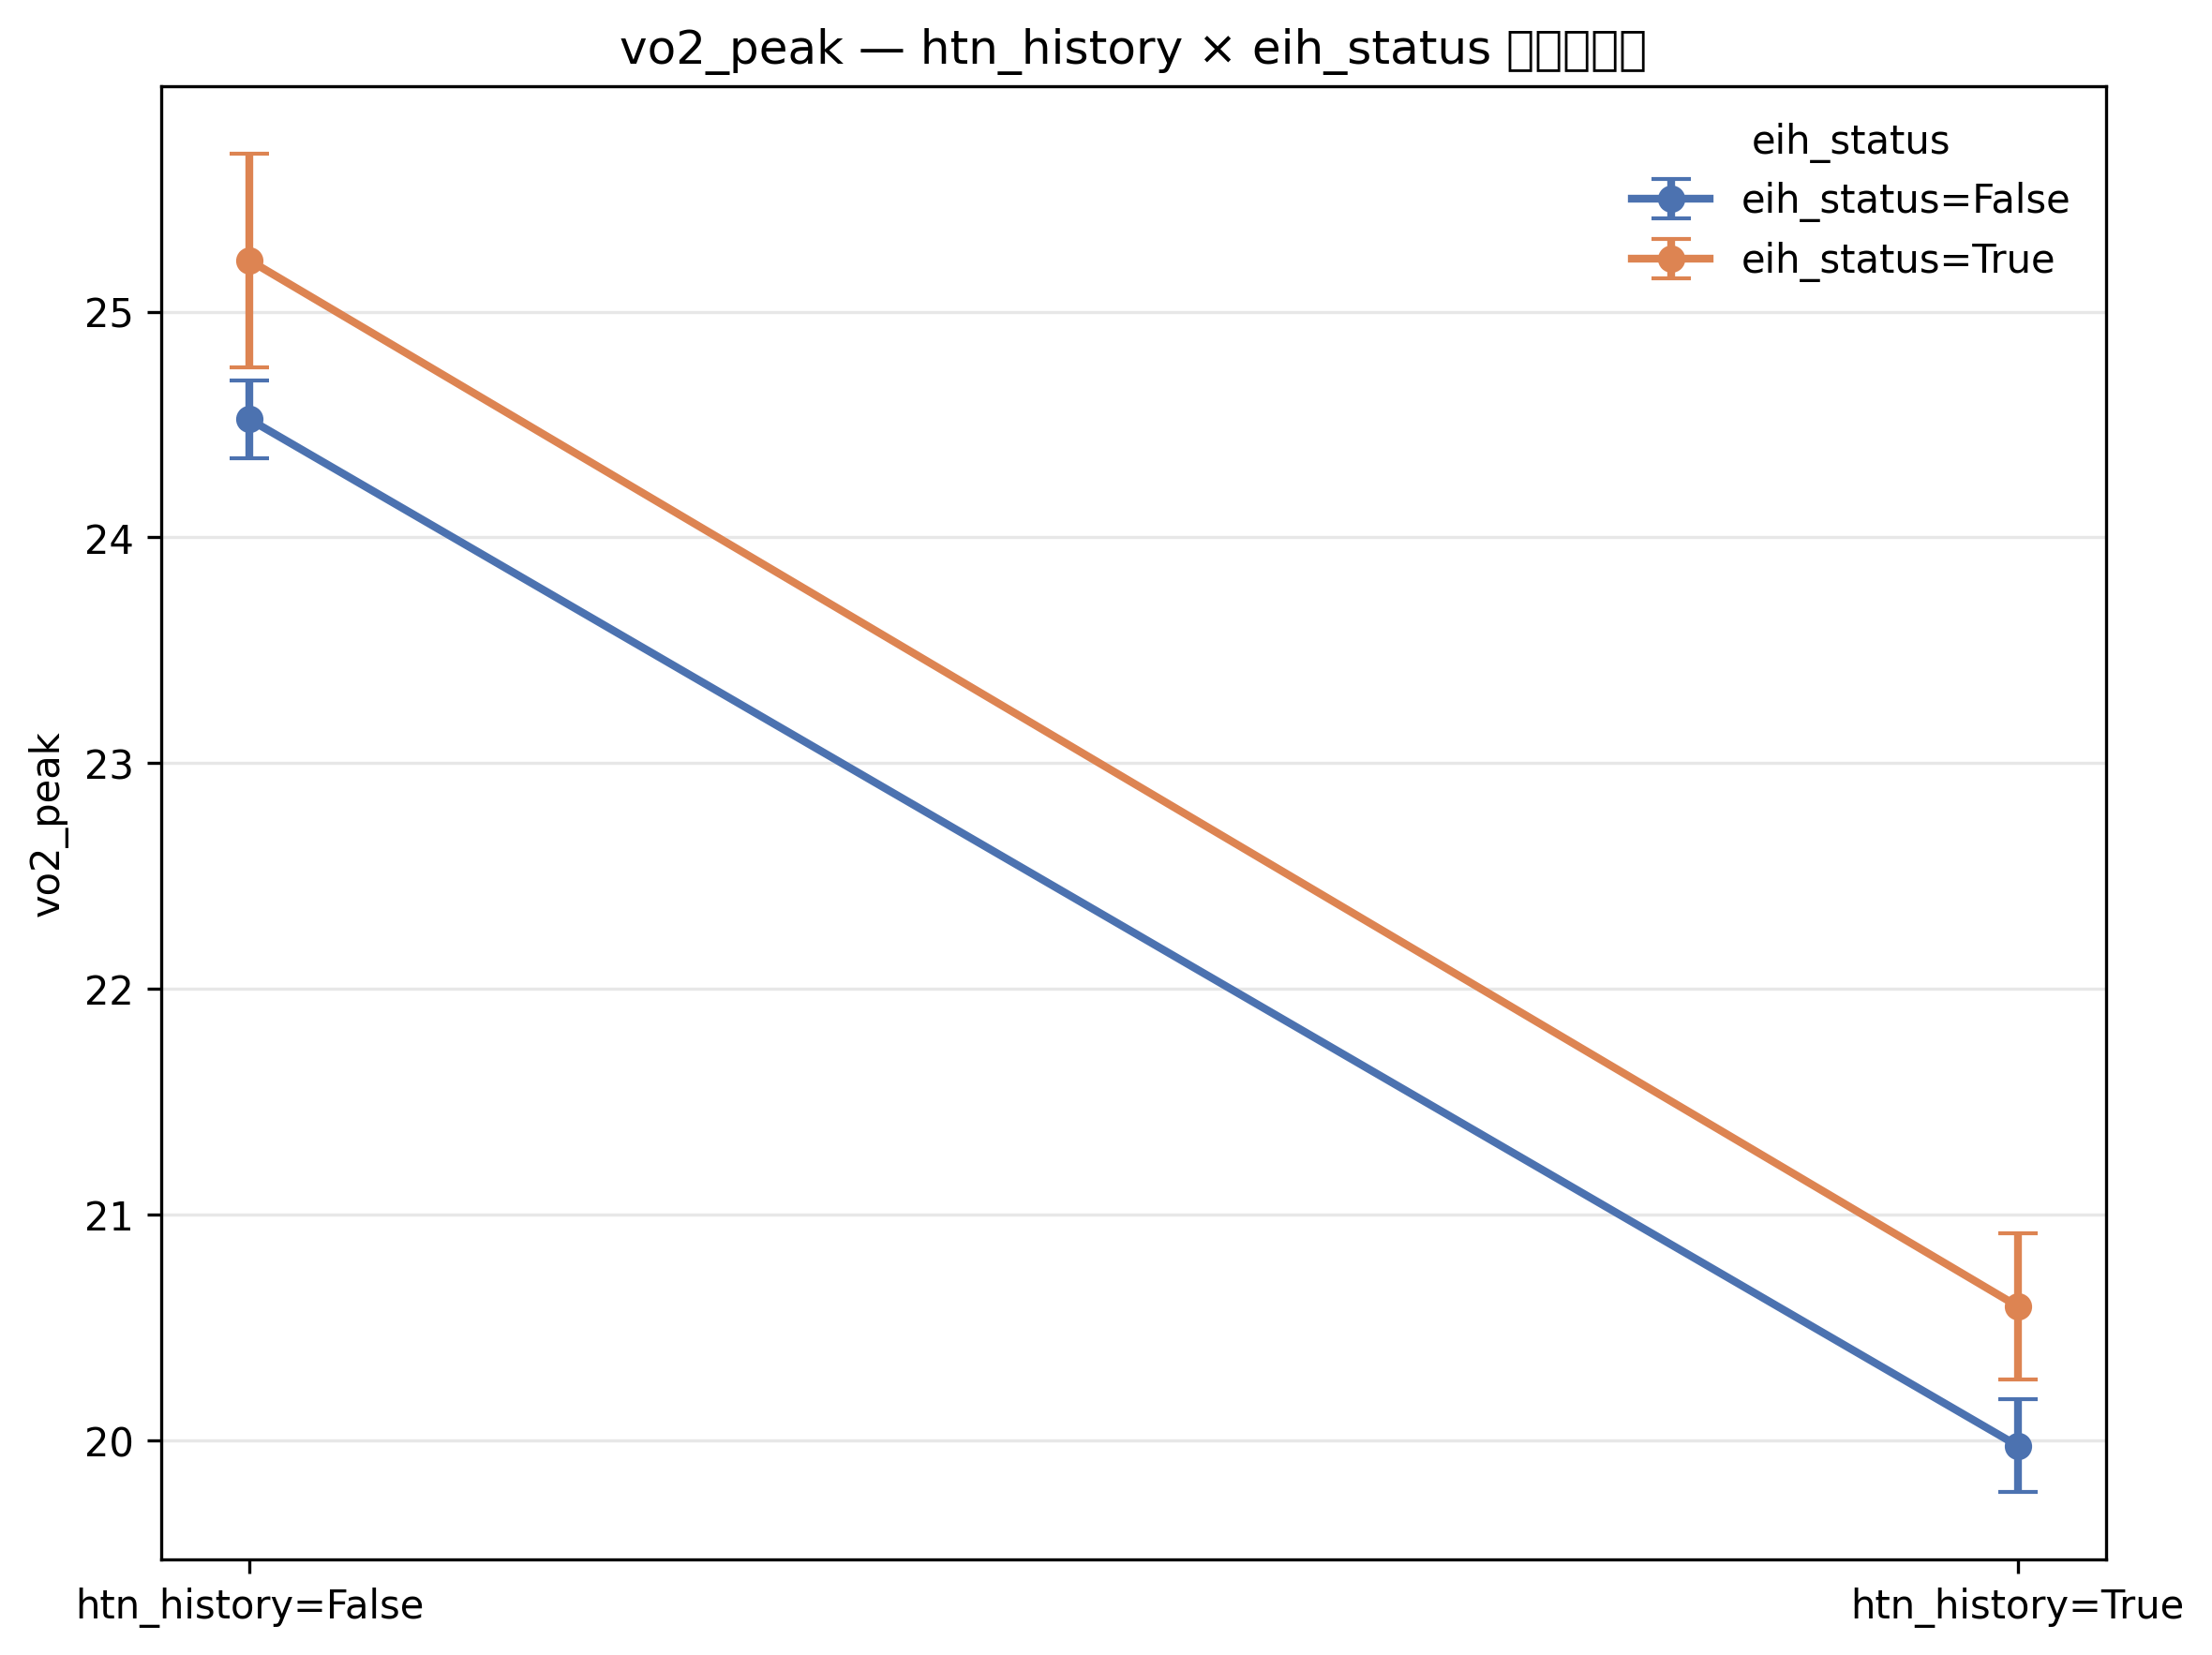
\includegraphics[width=0.85\textwidth]{figures/interaction_plots.png}
\caption{HTN$\times$EHT 双因素交互效应图（VO$_2$peak 分组均值）。
CTRL vs HTN 组差异显著（$\eta^2_p$=0.084，中等效应），
EHT 阳性/阴性组在相同 HTN 状态下 VO$_2$peak 相近，交互效应不显著（$p = 0.894$）。
此结果支持 Reserve 域（HTN 独立主效应）与即时不稳定层（EHT 独立主效应）的双层分离设计。}
\label{fig:interaction}
\end{figure}

\begin{figure}[htbp]
\centering
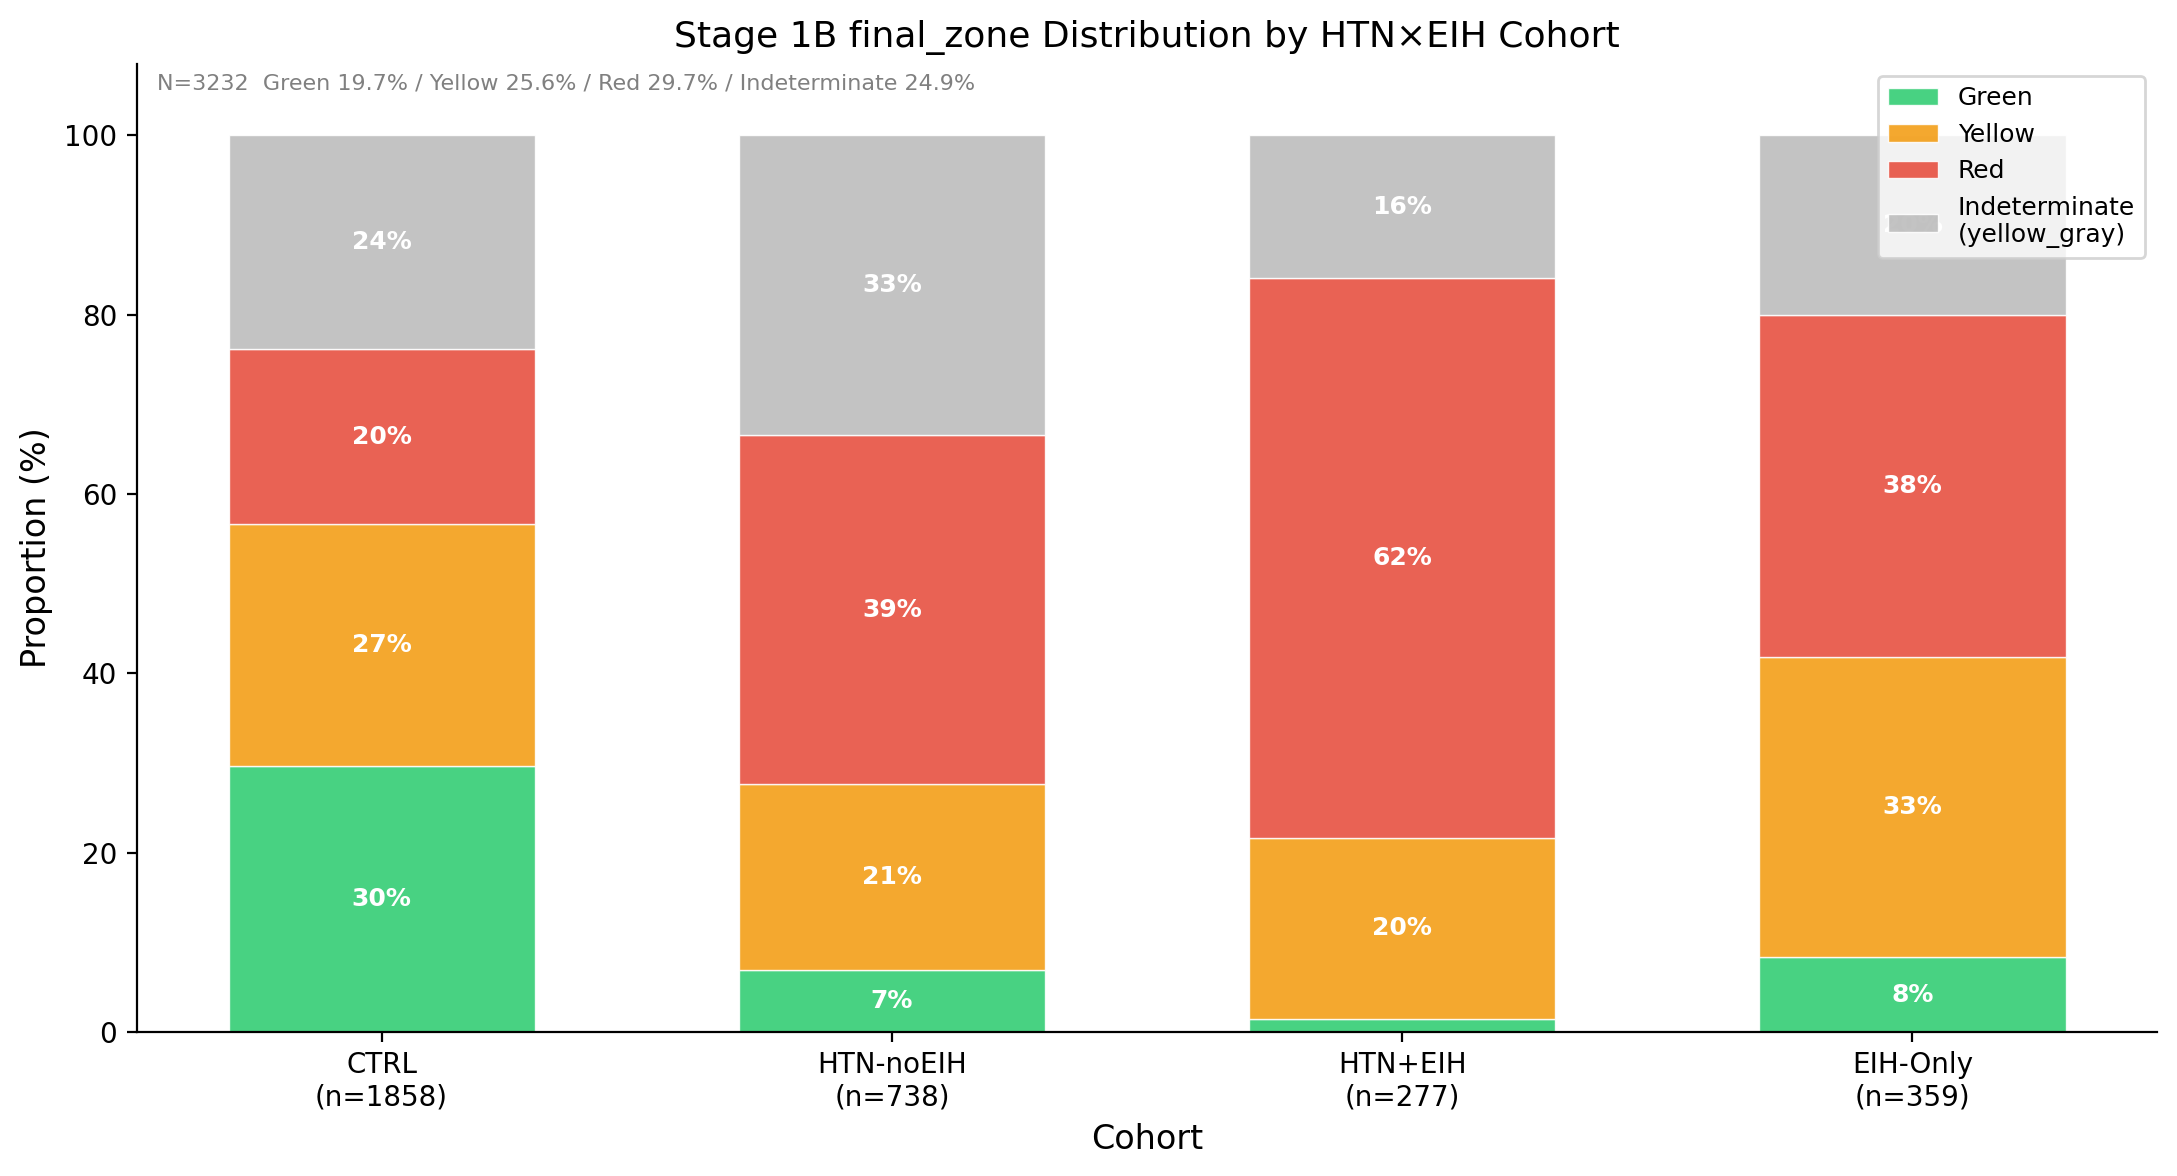
\includegraphics[width=0.85\textwidth]{figures/zone_distribution_stage1b.png}
\caption{最终安全分层分布（低危19.7\%/中危25.6\%/高危29.7\%/不确定层24.9\%）
按 HTN$\times$EHT 2$\times$2 队列（N=3,232）。
HTN-EHT 和 EHT-Only 组因严重不稳定覆盖规则（EHT阳性）触发，高危比例高于 CTRL 组；
高危来源：不稳定覆盖致高危220例（6.8\%）与表型负担致高危741例（22.9\%）。
不确定层24.9\%（805例），来源于置信度低于0.65且无严重不稳定的样本，反映 CPET 汇总指标固有的信息量局限。}
\label{fig:zone_dist_1b}
\end{figure}

\begin{figure}[htbp]
\centering
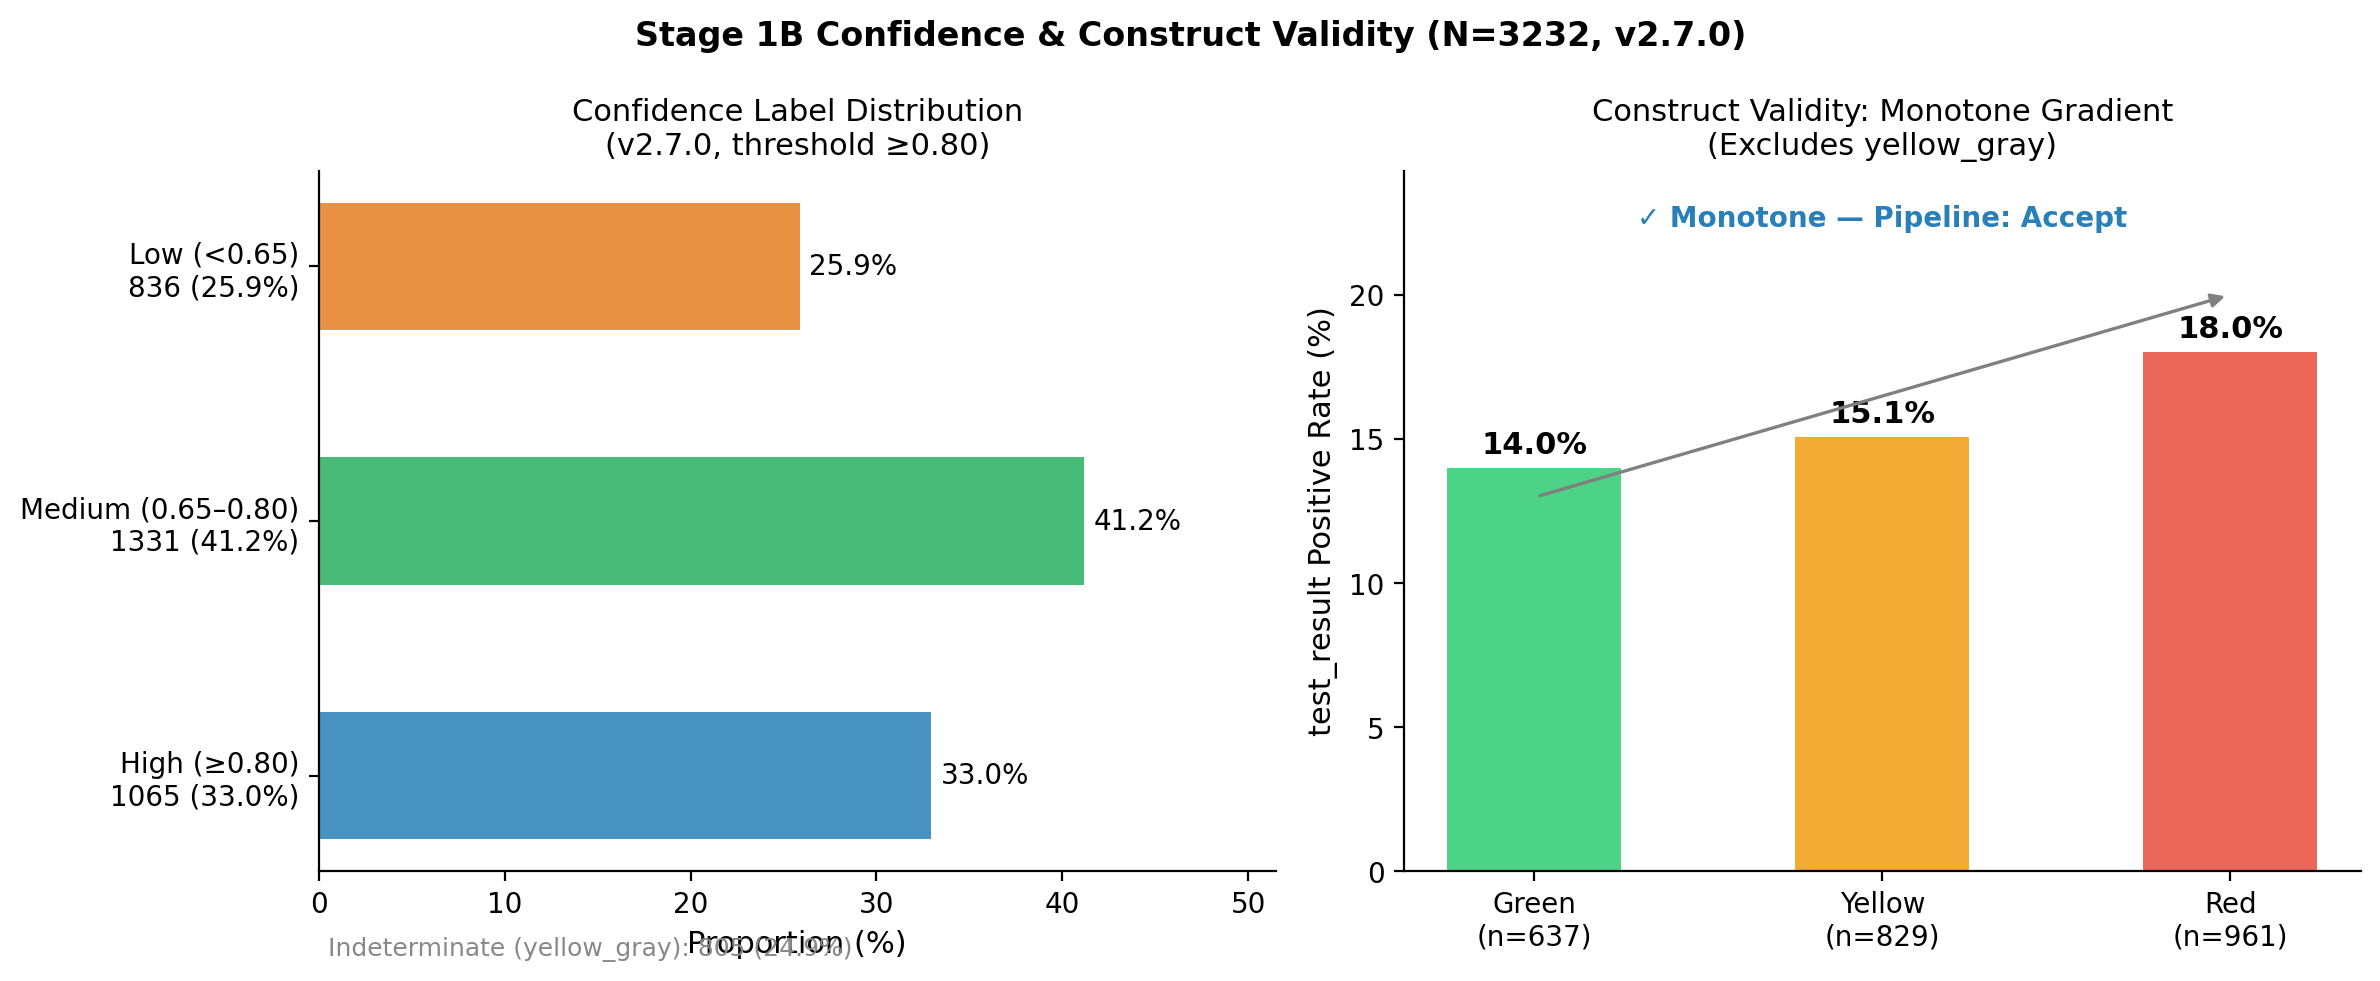
\includegraphics[width=0.95\textwidth]{figures/confidence_validity.png}
\caption{左：置信度标签分布（高置信度33.0\%/不确定层24.9\%，置信度阈值$\geq$0.80）。
右：最终安全分层对临床结局替代指标阳性率的单调梯度（低危14.0\% $<$ 中危15.1\% $<$ 高危18.0\%），
梯度方向正确，满足预设方法学质量标准。}
\label{fig:confidence_validity}
\end{figure}

% ============================================================
% 参考文献
% ============================================================
\bibliography{references}

\end{document}
